\documentclass[a4paper,11pt]{article}
\usepackage[utf8]{inputenc}
\usepackage[french]{babel} 
\usepackage[T1]{fontenc} 
\usepackage{textcomp}
\usepackage{amsmath,amssymb}
\usepackage{mathrsfs}
\usepackage{stmaryrd}
\usepackage{graphicx}
\usepackage[titlepage,fancysections]{polytechnique}

\title{SpeedTyper}
\author{Vincent DALLARD et Romain FOUILLAND}
\subtitle{Projet d'INF431}
\date{Mars 2018}


\begin{document}
\maketitle
\section{Introduction}
Le but du SpeedTyper est de taper le plus vite possible. Pour que le jeu soit pertinent, il faut donc que l'interface utilisateur (UI) soit la plus fluide possible. Ainsi, il faut gérer la vérification des mots et le décompte du temps en parallèle pour ne pas ralentir l'UI. De ce fait, un programme utilisant plusieurs threads est nécessaire.\par
Nous avons ainsi développée une première version naïve qui était gérée par l'UI. Afin d'améliorer les performances du jeu, nous avons dans une deuxième version utilisé des managers pour répartir les tâches et les nouveaux mots.\par

\section{Fonctionnement}
\subsection{Description}
La figure suivante est notre interface graphique finale.\par
\begin{center}
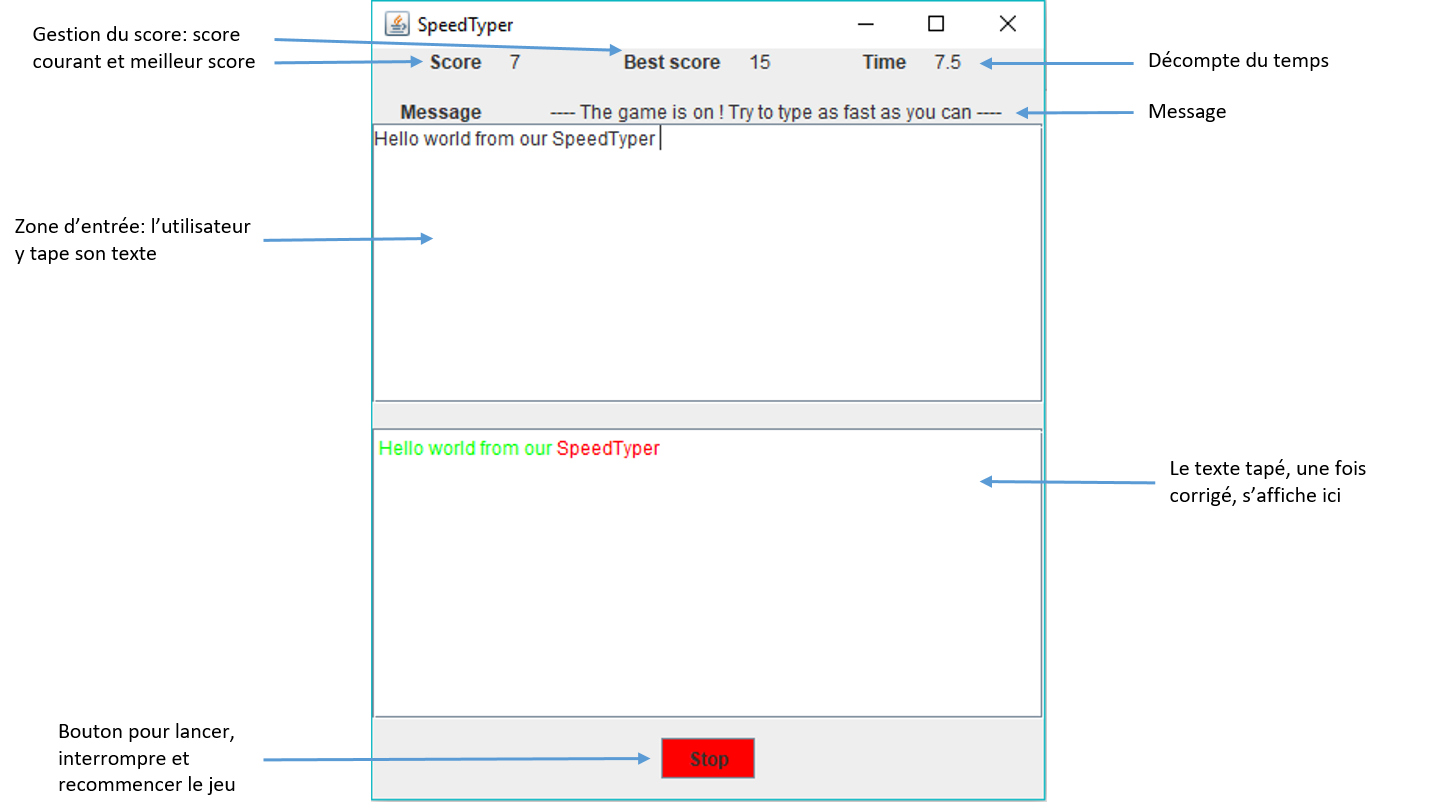
\includegraphics[width = 17cm, height = 11cm]{interfaceGraphique.png}
\end{center}\par
Pour l'interface utilisateur, on a choisi d'utiliser un JPanel. Cependant, la fenêtre s'affiche différemment sur nos ordinateurs et il peut donc être nécessaire de la redimensionner un peu pour voir tous les champs.\par
Comme on peut le voir, la première ligne sert à gérer les données du jeu à savoir :
\begin{itemize}
\item Le score courant du joueur
\item Le meilleur score qui est stocké dans un fichier en local pour être conservé entre les parties
\item Le temps restant avant le début du jeu ou la fin de la partie (une fois celle-ci lancée)
\end{itemize}\par
La ligne suivante permet d'afficher des messages pour donner des informations au joueur (le jeu va bientôt être lancé, le jeu est fini, en cours ou encore le meilleur score a été battu).\par
Les deux zones de texte sont la zone d'entrée où l'utilisateur pourra taper de la façon la plus fluide possible et la zone de sortie où le texte corrigé s'affiche en couleur :
\begin{itemize}
\item gris en attente de correction
\item vert si le mot existe en anglais
\item rouge s'il n'existe pas
\item gras et plus gros si c'est un nom des films célèbres
\end{itemize}\par
Enfin, un bouton permet de lancer ou arrêter la partie.
\subsection{Fonctionnalités}
Notre SpeedTyper permet d'interrompre et de relancer une nouvelle partie à tout moment en appuyant sur le bouton en bas.\par
Pour le test des mots, nous avons utilisé l'API Oxford Dictionnaries qui teste les mots en anglais avec une requête. Chaque mot correct rajoute sa longueur en points et l'enlève s'il n'existe pas.\par
Pour le test des noms de films, nous testons l'appartenance à une base de 250 films stockés dans un fichier texte. Un bon nom ajoute sa longueur au score (en comprenant les espaces pour compenser un titre avec que des mots faux).\par
\vspace{1cm}

\section{Implémentations}
\subsection{Version naïve}
Dans cette première version, le Thread Writer était chargé d'afficher l'UI et de gérer le texte tapé. Cependant, il devait aussi lancé le Timer et, à chaque fois qu'un nouveau mot était entré, il devait créer un Thread Checker qui devait tester ce mot.\par
Nous nous sommes dit que cette implémentation mettait trop de charge sur Writer et que cela pouvait rendre l'UI moins fluide que désirée.\par


\subsection{Threads managers}
\subsubsection{Chargement}
Lors de l'ouverture du jeu, un Thread manager \textit{EventDispatcher} est lancé et va s'occuper de lancer les bons Threads aux bons moments. Il commence par lancer l'UI et le Thread manager des entrées \textit{InputManager}. Ensuite, il charge les noms de films depuis un fichier texte local. Enfin, \textit{EventDispatcher} crée le Thread \textit{Timer} (mais ne le lance pas encore) qui va gérer le temps. Une fois tous ses chargements effectués, \textit{EventDispatcher} se met en attente de l'appui sur le bouton Go par l'utilisateur (par un \textit{await} sur la variable de condition \textit{goSignal}).\par
\subsubsection{Lancement du jeu}
Lorsque l'utilisateur appuie sur Go, l'UI envoie un signal sur \textit{goSignal} qui réveille \textit{EventDispatcher}. Celui-ci lance alors le timer qui décompte 3 secondes avant de permettre au joueur de taper du texte. Ensuite, il lance \textit{nbThreads} (que l'on a pris égal à 3) Threads \textit{Checker} qui vont être chargés de vérifier la validité des mots tapés en parallèle. Enfin, \textit{EventDispatcher} se rendort en attendant la variable de condition \textit{overSignal}.\par
De son côté, \textit{Timer} décompte 3 secondes avant de permettre à l'utilisateur de taper puis relance un décompte de la durée définie pour le jeu (dans \textit{Timer.duration} en ms).\par
\subsubsection{Déroulement du jeu} 
Pendant toute la durée du jeu, le Thread \textit{Writer} gère l'UI. En particulier, il empêche l'utilisateur de supprimer les mots déjà validés et récupère le dernier mot à chaque fois que l'utilisateur appuie sur la touche \textit{espace}. Il écrit ce mot dans une \textit{LinkedBlockingQueue} partagée avec \textit{InputManager} qui lui va ensuite se charger de gérer les mots pour laisser \textit{Writer} libre de s'occuper de l'UI.\par
À chaque fois qu'il récupère un mot, \textit{InputManager} va :
\begin{itemize}
\item l'écrire dans une \textit{LinkedBlockedQueue} partagée avec les Threads \textit{Checker}. Cela réveille un Thread \textit{Checker} qui va envoyer une requête à l'API pour tester la présence du mot. En fonction du résultat, il va mettre à jour le score et la couleur du mot dans la fenêtre de sortie.
\item créer et lancer un Thread \textit{MovieChecker}. Ce dernier va parcourir la liste des films pour voir si des films commencent par le mot tapé. Si cela n'est pas le cas, il s'arrête. Dans le cas contraire, il s'endort et attend que l'\textit{InputManager} ait traité un nouveau pour se réveiller et traiter le titre correspondant à la concaténation des deux mots. Il répète ces actions jusqu'à tomber sur un des 250 titres ou jusqu'à n'avoir plus aucun des titres qui pourrait correspondre (il s'arrête).
\end{itemize}
\subsubsection{Fin}
Deux scenarii sont envisageables pour finir le jeu :
\begin{itemize}
\item Soit le compte à rebours du \textit{Timer} arrive à 0. Dans ce cas, il envoie un signal sur \textit{overSignal} avant de mettre à jour le meilleur score le cas échéant. Ce signal réveille \textit{EventDispatcher} qui va recréer un nouveau \textit{Timer} et attendre un nouveau un appui sur le bouton Go.
\item Soit le joueur appuie sur le bouton Stop. Dans ce cas, il ne compte plus écrire donc le Thread \textit{Writer} lui-même peut se charger d'envoyer un signal \textit{overSignal} et d'interrompre le \textit{Timer}.
\end{itemize}
\section{Analyse de la programmation concurrente}
\subsection{Verrous}
Pour pouvoir mettre à jour en parallèle le score (par les \textit{Checker} et les \textit{MovieChecker}) et le texte de sortie (écriture du mot en gris, puis de sa correction par un \textit{Checker} et éventuellement de sa correspondance avec un titre par un \textit{MovieChecker}), il fallait verrouiller ces champs. On a pour cela utilisé le mot-clé \textit{synchronized}.\par
Pour que l'\textit{InputManager} puisse réveiller les Threads \textit{MovieChecker} qui attendaient de nouveaux mots pour compléter leur titre, on a utilisé les mots-clés \textit{synchronized, notifyAll} et \textit{wait} sur la liste des mots traités par l'\textit{InputManager}.
\subsection{Signaux}
Pour signaler aux Threads concernés que le jeu vient d'être lancé (pour lancer le décompte) ou qu'il vient de se finir (relancer \textit{EventDispatcher}), on a utilisé un verrou et deux signaux \textit{signalGo} et \textit{signalOver} liés à ce verrou.
\subsection{Sleep}
Le \textit{Timer} ne peut jamais être arrêté car il doit mettre à jour le temps toutes les 0.1s mais on a mis un \textit{Thread.sleep(50);} tant qu'il restait plus de 300ms pour permettre d'éviter de l'attente active inutile.
\subsection{LinkedBlockingQueue}
On a utilisé une première \textit{LinkedBlockingQueue} pour dialoguer entre l'UI et l'\textit{InputManager}. Ce dernier dialogue avec les \textit{Checker} avec une autre \textit{LinkedBlockingQueue} car ces derniers sont en nombre fixe et ne meurent jamais pendant une partie.\par
Pour les \textit{MovieChecker}, on a choisi d'en créer autant qu'il peut y avoir de titres possibles en parallèle et de les tuer que lorsqu'il est impossible que leur séquence de mots corresponde à un titre. De ce fait, ils sont \textit{synchronized} sur la liste des mots traités par l'\textit{InputManager} et celui-ci leur envoie une \textit{String END\_OF\_GAME} pour les arrêter lorsqu'une partie est finie.
\end{document}
